%
% Шаблон для НИР
%

\documentclass[a4paper,12pt]{article}
\usepackage[backend=biber,sorting=none]{biblatex} % библиография
\usepackage{mathtext} %русские буквы в формулах
\usepackage[T2A]{fontenc}
\usepackage[utf8]{inputenc}
\usepackage[russian]{babel}
\usepackage{amsmath}
\usepackage{fancyvrb}
\usepackage{formular}
\usepackage{setspace} % управление междустрочными интервалами
%поля документа
\usepackage[left=3cm,right=1cm,top=2cm,bottom=2cm]{geometry}

\usepackage{misccorr} % точки в конце номеров разделов, использовать перед пакетом ccaption!
\usepackage{ccaption} % изменения подписей к рисункам и табл.
% отступ перед первым абзацем
\usepackage{indentfirst}
%вставка изображений
\usepackage{graphicx}
% счетчики
\usepackage{totcount}
% управление содержанием
\usepackage{tocloft}
% управление таблицами и рисунками
\usepackage{float}

%для добавления количества источников в реферат
\newtotcounter{citnum} %From the package documentation
\def\oldbibitem{} \let\oldbibitem=\bibitem
\def\bibitem{\stepcounter{citnum}\oldbibitem}

% окружение для листингов - с нумерацией строк слева
\DefineVerbatimEnvironment{MyCode}{Verbatim}{frame=lines,numbers=left,numberblanklines=false,framesep=5mm}

% автоматическая нумерация листингов
\newfloat{Program}{phb}{lop}
\floatname{Program}{Листинг}
\floatstyle{ruled}

\setcounter{secnumdepth}{3} % глубина нумерации до подразделов

%если нужны точки в оглавлении для разделов - раскомментируйте следующую команду
%\renewcommand{\cftsecleader}{\cftdotfill{\cftdotsep}}

\addto\captionsrussian{
\renewcommand{\figurename}{Рисунок}
\renewcommand{\tablename}{Таблица}
}

% дефис в подписи к рисункам
\captiondelim{ -- } 

% Настройки для окружений с подчеркиваниями для подписей и пр.
\setFRMfontencoding{T2A}
\setFRMdfontencoding{T2A}
% thanks to A.Starikov
\setFRMfontfamily{cmr}
\setFRMdfontfamily{ptm}
\setFRMdfontsize{10pt}

% задает длину поля для подписи на титульной странице
\newFRMfield{xtitlesign}{40mm}

% поле для факультета или кафедры
\newFRMfield{fcath}{65mm}


\addbibresource{rbiblio.bib}

\begin{document}

% счетчики страниц, рисунков, таблиц
\regtotcounter{page}
\regtotcounter{figure}
\regtotcounter{table}

\renewcommand{\refname}{\centerline{СПИСОК ИСПОЛЬЗОВАННОЙ ЛИТЕРАТУРЫ}} 
\renewcommand{\contentsname}{\centerline{СОДЕРЖАНИЕ}} 
%\renewcommand{\refname}{Список источников}  % По умолчанию "Список литературы" (article)
%\renewcommand{\bibname}{Литература}  % По умолчанию "Литература" (book и report)

% титульная страница
\thispagestyle{empty}
\begin{center} \small
\textbf{МИНИСТЕРСТВО ОБРАЗОВАНИЯ И НАУКИ РОССИЙСКОЙ ФЕДЕРАЦИИ}\\
ФЕДЕРАЛЬНОЕ ГОСУДАРСТВЕННОЕ АВТОНОМНОЕ ОБРАЗОВАТЕЛЬНОЕ УЧРЕЖДЕНИЕ
ВЫСШЕГО  ОБРАЗОВАНИЯ\\
«Национальный исследовательский ядерный университет «МИФИ»\\
\textbf{Обнинский институт атомной энергетики} – \\
филиал федерального государственного автономного образовательного учреждения высшего\\
образования «Национальный исследовательский ядерный университет «МИФИ»\\
(ИАТЭ НИЯУ МИФИ)
\end{center}
\vfill
\medskip

% Направление подготовки следует уточнять,
% магистры и бакалавры могут иметь разные наименования
\begin{center}
\begin{tabular}{rl}
Отделение & \useFRMfield{fcath}[\large Интеллектуальных кибернетических систем] \\ 
Направление подготовки & \useFRMfield{fcath}[\large Информационные системы и технологии] \\ 
\end{tabular} 
\end{center}

\vfill

\large 

\begin{center}
	Научно-исследовательская работа \\
	
	\medskip
	
	\textbf{\Large 
		Построение системы учета семейного бюджета с использованием QT Framework
	}
	
\end{center}

\vspace{1cm}

\begin{tabular*}{\textwidth}{lcr}
Студент группы ИС-Б14-З & \useFRMfield{xtitlesign} & А.В. Миронов\\
& & \\
Руководитель & & \\
к.т.н., доцент & \useFRMfield{xtitlesign} & О.А. Мирзеабасов
\end{tabular*}


\vfill
\large

\begin{center}
Обнинск, 2018
\end{center}

\onehalfspacing

\pagebreak

% реферат
\thispagestyle{empty}

\section*{\centering РЕФЕРАТ}

% возможно, кол-во источников придется вставлять вручную
\total{page} стр., \total{table} табл., \total{figure} рис. , \total{citnum} ист. 

\pagebreak
\thispagestyle{empty}


\section*{\centering ОБОЗНАЧЕНИЯ И СОКРАЩЕНИЯ}


\pagebreak



\tableofcontents
% если нужно добавить "Стр." над номерами страниц - раскомментируйте следующую команду
%\addtocontents{toc}{~\hfill\textbf{Стр.}\par}

\pagebreak

\section*{\centering ВВЕДЕНИЕ}
\addcontentsline{toc}{section}{ВВЕДЕНИЕ}


Обработка данных с помощью различных языков программирования приобретает всё большую популярность с каждым годом. Одним из языков для статистической обработки и визуализации данных является \textbf{R}. В языке \textbf{R} существуют пакеты для визуализации и вычисления траекторий динамических систем. 

Задачи, решаемые в ходе работы (в соответствии с заданием на НИР):

\begin{enumerate}
    \item что-то сначала
    \item что-то потом
    \item подготовка отчета. 
	
\end{enumerate}
 % текст введения в файле intro.tex
\pagebreak

%\input{Post_zad}
\pagebreak
% первая глава

\section{Название первого раздела}

\subsection{Таблицы}

Текст подраздела посвящен таблице~\ref{tab:t1}

\begin{table}[H]
\caption{Пример таблицы}
\label{tab:t1}
\begin{center}
\begin{tabular}{|r|p{5.5cm}|p{2.5cm}|}
\hline 
1 & Первый текст в ячейке фиксированной ширины & $E=mc^2 $ \\ 
\hline 
12 & Второй текст тоже может быть произвольно длинным & $\sin \pi = 0 $ \\ 
\hline 
\end{tabular} 
\end{center}
\end{table}

\subsection{Вставка изображения}

\begin{figure}[H]
	\centering
	\includegraphics[width=0.7\linewidth]{pics/pic3D}
	\caption{Пример изображения для демонстрации возможности вставки в документ}
	\label{fig:pic3d}
\end{figure}



Изображение на рис.~\ref{fig:pic3d} находится в подкаталоге pics.

  % первая глава - в файле part1.tex
\pagebreak
% второй раздел - файл part2.tex

\section{Методики учета семейного бюджета}

\subsection{Где вести учет семейного бюджета}

\subsubsection{Тетрадь или амбарная книга}
Несомненно, что для вычислений, связанных с учетом личных финансов,
было бы удобно воспользоваться компьютером и вести в нем все записи, однако если такой возможности нет, то можно завести тетрадь или амбарную
книгу. В самом простом обобщенном случае рекомендуется разбить лист на
три графы:
\begin{table}[H]
\caption{Пример теблицы для учета семейного бюджета}
\label{tab:t1}
\begin{center}
\begin{tabular}{|r|p{5.5cm}|p{2.5cm}|}
\hline 
Доход & Расход & Итого \\ 
\hline 
 &  &  \\ 
\hline 
\end{tabular} 
\end{center}
\end{table}

Графы Расход и Доход будут отражать соответствующее движение
денег вашего кошелька, а графа Итого нужна для того, чтобы сверять цифры на бумаге с количеством денег в карманах. Как ни странно, они должны
совпадать.
Такой подход в целом приемлем для одного человека, он даже позволит
отследить и выявить необязательные расходы, которые впоследствии можно
уменьшить или вовсе убрать. Однако в таком виде о какой-либо наглядности
и систематизации говорить не приходится. Тем более в рамках рассмотрения
бюджета семьи. Ведь, как уже говорилось в предыдущей части, семейный
бюджет охватывает множество составляющих.
Для повышения наглядности и хоть какой-то систематизации доходов и
расходов, приведенную табличку необходимо разбавитьї дополнительными
колонками группируя разные виды расходов в соответствии реально имеющимся.
Например, в первую колонку можно записывать коммунальные платежи,
свет, интернет или аренду. Во второй колонке записывать лишь траты на
продукты питания, в третьей личные расходы, в четвертой расходы на развлечения и в пятой непредвиденные расходы.
Естественно, существующую таблицу нужно модернизировать под себя и
вероятно кто-то посчитает нужным добавить колонки по бытовой химии, уходу за кошкой, ребенком, родителями и т.д.
Эти расширения, в конце концов, приведут к тому, что таблица попросту
перестанет умещаться даже в амбарную книгу. И в этом случае на помощь
приходят компьютерные программные средства.

\subsubsection{Электронные таблицы}
Более продвинутый путь, приступить к ведению семейного бюджета при
помощи электронной таблицы (Excel, Google Docs и т.п.), где уже даже имеются основные формулы для анализа бюджета. По сути, вам остается лишь
выбрать и применить их к своим данным. Но и тут есть путь проще.
Дело в том, что на сегодняшний день существует множество специальных
шаблонов для электронных таблиц, в которых уже учтены некоторые наиболее популярные поля и необходимые для расчетов формулы.
\subsubsection{Специализированные программы}
Кроме шаблонов для табличных редакторов, в сети интернет предлагается
масса специальных программ для ведения учета и планирования семейного
бюджета.
Они позволяют автоматизировать большую часть работы, что значительно
упрощает процесс ведения домашних финансов.
Помимо того, эти программы, как правило, имеют массу вспомогательных функций, которые позволяют выявить слабые и сильные стороны вашего отношения с деньгами, помогут явно обратить внимание на, казалось бы,
очевидные, вещи, но почему-то не используемые в повседневной жизни. По
сути, программы для ведения семейного бюджета значительно облегчают и
помогают создать целостную картину наших взаимоотношений с финансами.
 % вторая глава - в файле part2.tex
\pagebreak
% !TeX spellcheck = de_DE
\part{Выбор инструментов и средств разработки}
\section{Обзор и выбор СУБД}
\subsection{СУБД MySQL}
MySQL — свободная реляционная система управления базами данных. Разработку и поддержку MySQL осуществляет корпорация Oracle, получившая права на торговую марку вместе с поглощённой Sun Microsystems, которая ранее приобрела шведскую компанию MySQL AB. Продукт распространяется как под GNU General Public License, так и под собственной коммерческой лицензией. Помимо этого, разработчики создают функциональность по заказу лицензионных пользователей.\cite{mysql}\\
\subsection{СУБД SQLite}
SQLite — это встраиваемая кроссплатформенная БД, которая поддерживает достаточно полный набор команд SQL и доступна в исходных кодах (на языке C). Исходные коды SQLite находятся в public domain, то есть вообще никаких ограничений на использование.\\
\subsection{Обоснование выбора СУБД}
Для наибольшего удобства была использована SQLite, что позволило достаточно сильно ускорить скорость открытия потребления, а также существенно снизить потребляемое количество оперативной памяти. В ранних версиях программы при наличии большого количества записей в базе данных программа пыталась полностью перенести данные в память, что приводило к общему замедлению работы операционной системы и возможному повреждению данных.

\section{Обзор и выбор языка программирования}
При выборе языка программирования для создания приложения я остановился на трех базовых концепциях:

\begin{enumerate}
	\item Портируемость
	\item Легкость
	\item Удобство использования
	\item Большие возможности
\end{enumerate}

Благодаря этому списку мне удалось достаточно сильно сократить число
языков программирования на которых можно было написать приложение, в
итоге я остановился на языке

C++ с расширением QT Framework. Который оказался достаточно комфортным и легко расширяемым для выполнения необходимых задач.

\part{Разработка базы данных для хранения информации}
\section{Проектирование базы данных}
База данных состоит из 1 таблицы имеющую создающуюся с помощью следующего запроса:
\begin{MyCode}
	CREATE TABLE  IF NOT EXISTS "operations"(
	"id" INTEGER  PRIMARY KEY  NOT NULL ,
	"time" DATETIME DEFAULT (CURRENT_TIMESTAMP),
	"summ" NOT NULL  DEFAULT (null),
	"comment"  NOT NULL,
	"catid" INTEGER DEFAULT (null),
	"side" BOOL DEFAULT (0))
\end{MyCode}

\section{Реализация базы данных в СУБД SQLite}
Таблица создается в базе данных при запуске программы используя запрос указанный выше\\
 % третья глава - в файле part3.tex
\pagebreak
\part{Разработка програмного обеспечения}

Как правило систематическое занесение доходов и расходов в таблицу, а
также подсчет итогового баланса может оказаться весьма непростым занятием, но и использование электронных таблиц и специализированных программ
тоже не тривиальная задача, поскольку такие методы разрабатываются с учетом максимально широких возможностей использования, от самых простых
табличных расчетов и до учета дивидендов от приобретенных акций, что не
очень хорошо ложится на базовый семейный бюджет.

\section{Разработка базовой концепции приложения}
В качестве базовой концепции приложения был выбран вариант модифицированных электронных таблиц. Самым простым вариантом была следующая структура
\begin{enumerate}
	\item Размер операции
	\item "Сторона"операции (приход/расход)
	\item Коментарий к операции
	\item Дата и время операции
\end{enumerate}

Остаток вычислялся путем последовательного суммирования (с модификатором "стороны") размеров операции отсортированных по датам и времени
операции

\subsection{Начало разработки}
Первоначальная версия сущестовала в консольном виде без взаимодействия с курсором мыши. Данные хранились в текстовом виде, что позволяло
легко модифицировать записанные данные. Позже были добавлены категории записей, которые позволили однозначно делать подсчет расходов по категориям расходов.

\section{Разработка графической версии}
Немного позже был разработан первоначальный вариант графической версии приложения, он по прежнему записывал данные в файл и при этом работал достаточно неэффективно.

\begin{figure}[H]
	\centering
	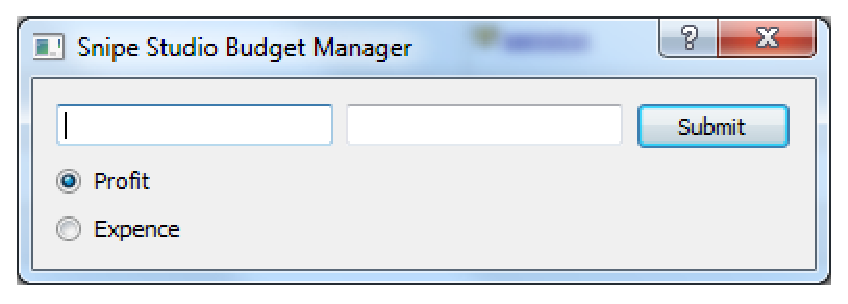
\includegraphics[width=0.7\linewidth]{pics/firstVersion.eps}
	\caption{Первоначальный вариант графического приложения Budget Manager}
	\label{fig:firstVersion}
\end{figure}

Немного позднее было добавлено поле отображающее список операций

\begin{figure}[H]
	\centering
	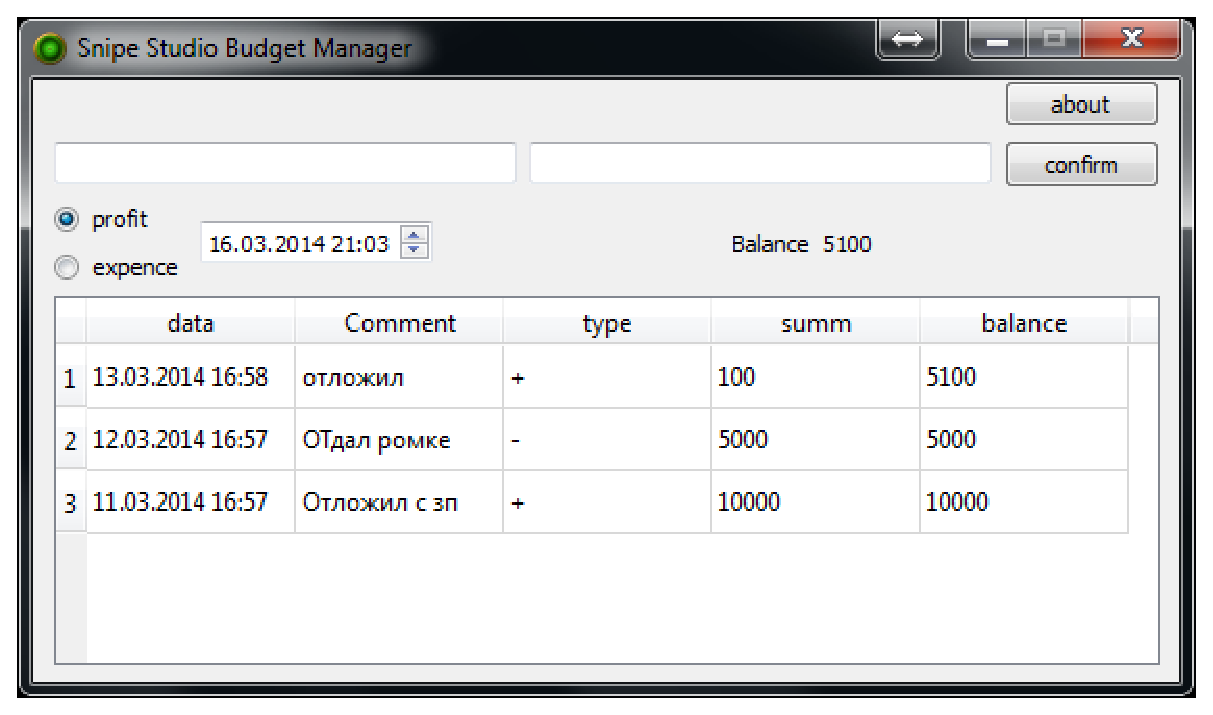
\includegraphics[width=0.7\linewidth]{pics/secondVersion.eps}
	\caption{Вариант графического приложения Budget Manager с таблицей со списком
		операции}
	\label{fig:secondVersion}
\end{figure}

Дальше был изменен метод хранения и изменения уже существующих записей, добавлено полноценное меню настроек, строки таблицы теперь окрашиваются в зависимости от выбраной "стороны"(приход/расход) для операции

\begin{figure}[H]
	\centering
	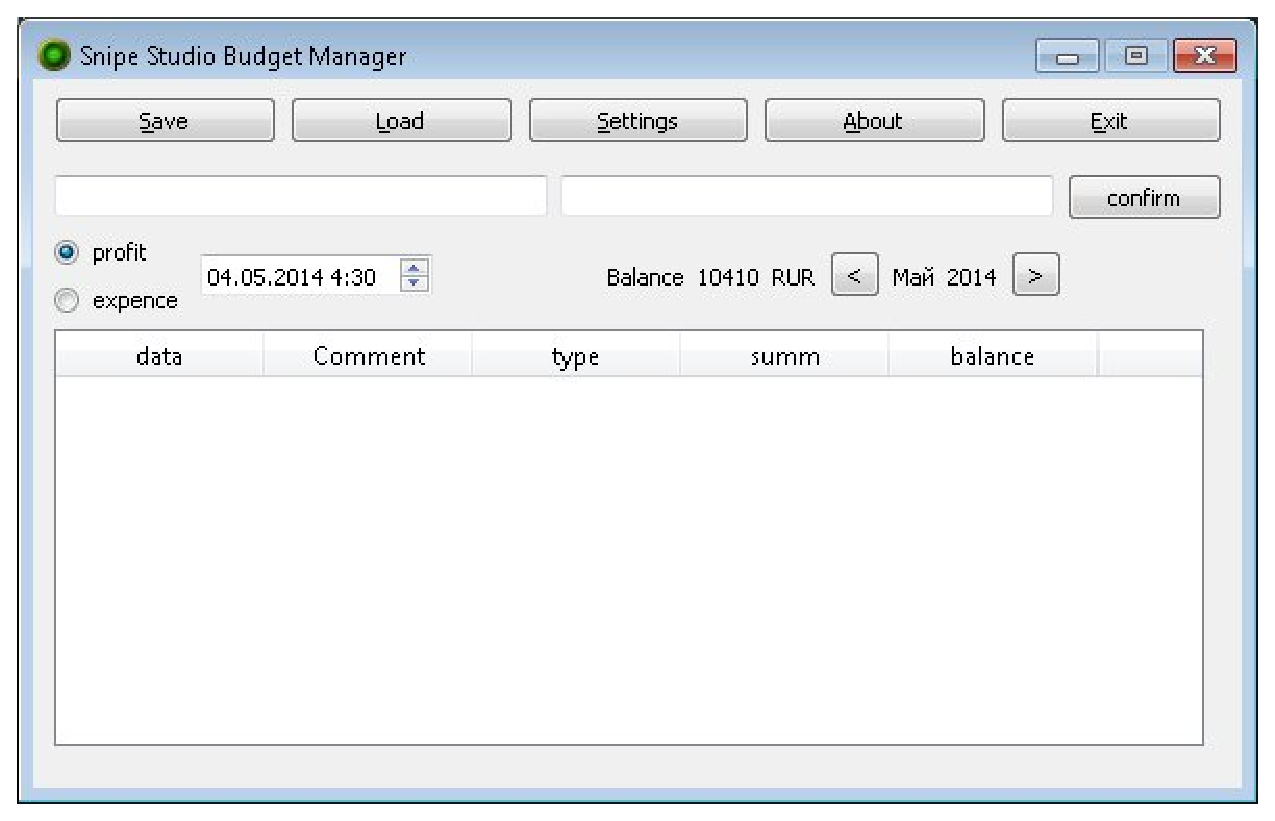
\includegraphics[width=0.7\linewidth]{pics/view1.eps}
	\caption{Окончательный вариант графического приложения Budget Manager}
	\label{fig:view1}
\end{figure}

Позже был изменен общий графический дизайн приложения 	и стал следующим:

\begin{figure}[H]
	\centering
	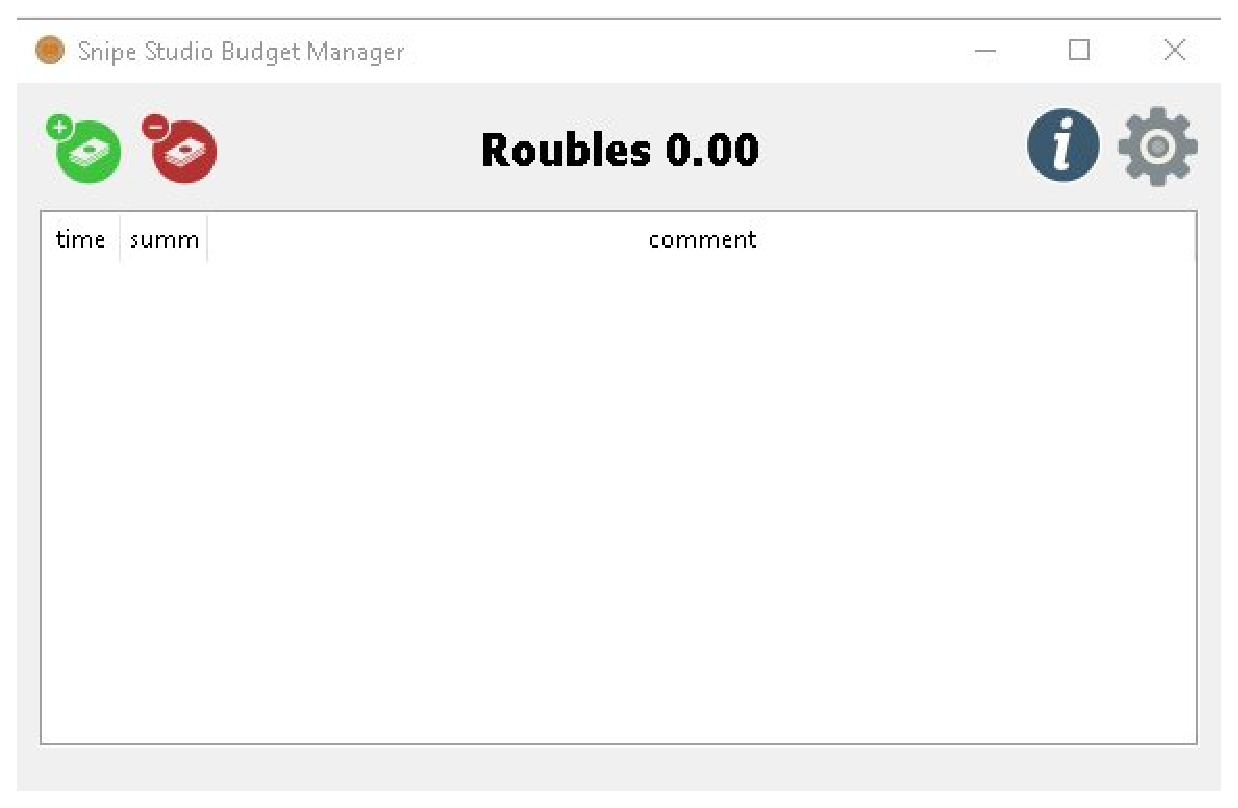
\includegraphics[width=0.7\linewidth]{pics/view2.eps}
	\caption{Второй вариант графического приложения Budget Manager}
	\label{fig:view2}
\end{figure}

Так же была собрана версия для Android

\begin{figure}[H]
	\centering
	
	\includegraphics[height=0.7\linewidth]{pics/viewAndroid.eps}
	\caption{Версия для Android}
	\label{fig:viewAndroid}
\end{figure}

\section{Автоматизированная сборка и тестирование}
Спустя некоторое время мне понадобилось автоматически собирать инсталляторы для каждого коммита, чтобы не тратить каждый раз время на полноценную сборку инсталлятора и deb-пакета для приложения. Для этих целей я выбрал Azure DevOps, который предоставлял бесплатные сборочные машины и целую готовую инфраструктуру для автоматизированной сборки и тестирования.\\
Для целей автоматизированного тестирования был создан интерфейс командной строки, который позволяет использовать все возможности приложения без необходимости запускать графический интерфейс пользователя, что позволило тестировать приложения в операционных системах без графической среды пользователя.\\
\subsection{Автоматическая сборка}
Сборочная цепочка для AzureDevops под операционную систему Linux на базе Ubuntu 16.04 имеет следующий вид:
\begin{figure}[H]
	\centering
	\includegraphics[width=1\linewidth]{pics/AzurePipeline.eps}
	\caption{Azure Pipeline}
	\label{fig:AzurePipeline}
\end{figure}

В шаге Install Prereqs происходит установка QT для возможности сборки приложения.\\
Prepare Sources заменяет версию в Файле appinfo.h на текущую версию приложения, т.е. имеет вид 0.8.3.(buildNumber)\\
Шаг Build осуществляет сборку бинарного файла приложения\\
Шаг GitHub Release публикует PreRelease версию на GitHub с указанием тага текущей сборки\\
\begin{figure}[H]
	\centering
	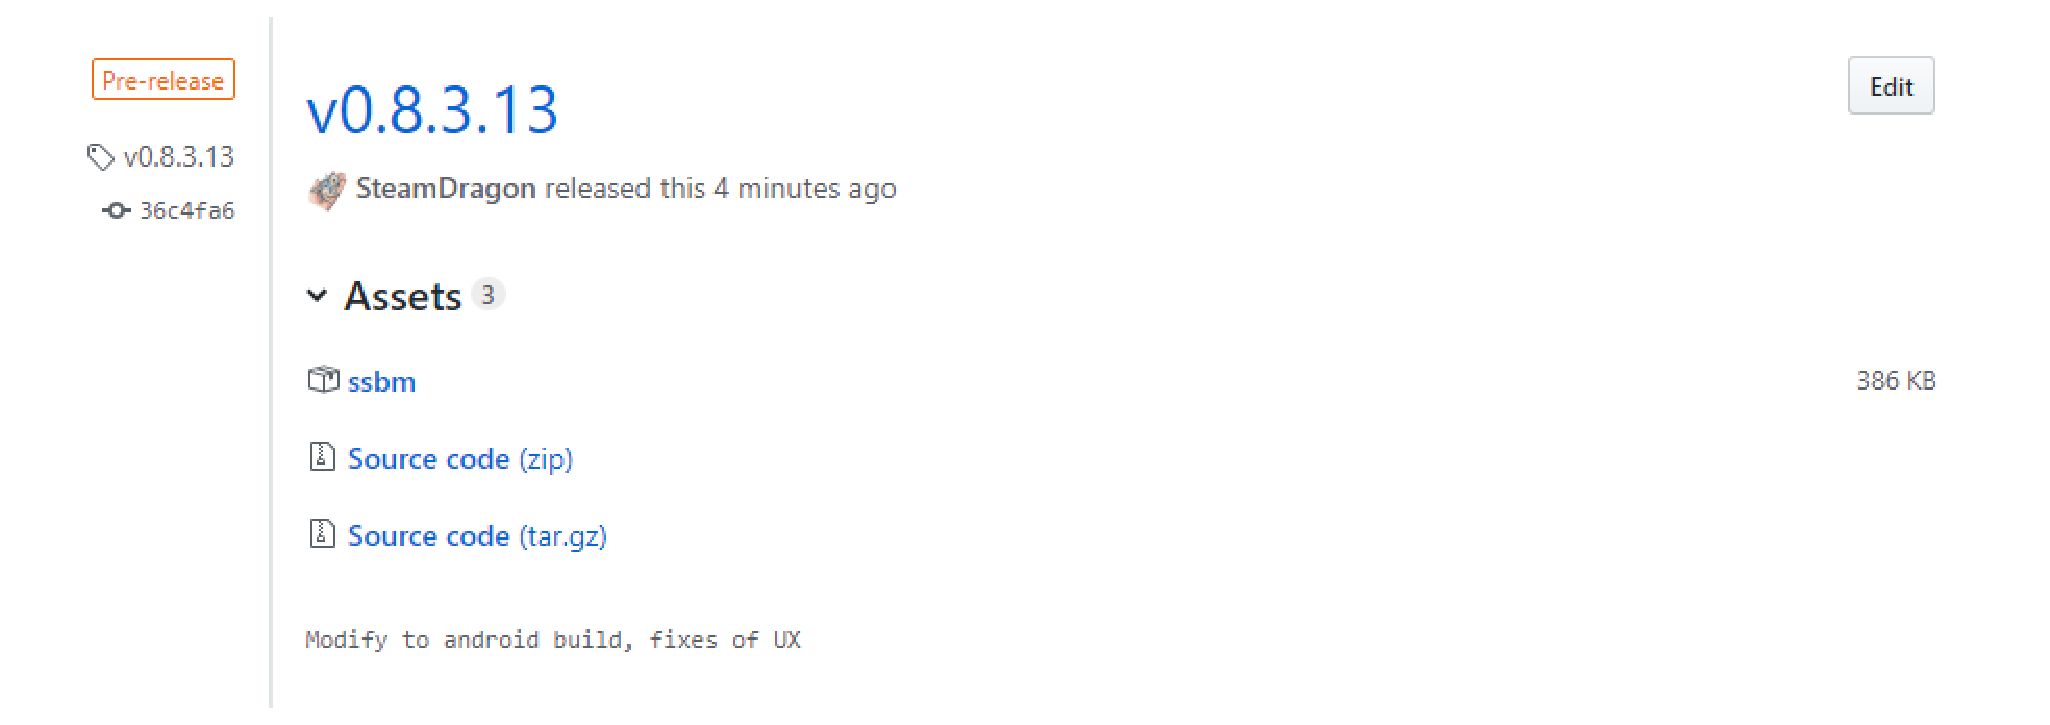
\includegraphics[width=1\linewidth]{pics/GHRelease.eps}
	\caption{Github Release}
	\label{fig:GHRelease}
\end{figure}
Сборка под операционную систему Windows имеет ту же структуру, что и сборка под Ubuntu, за одним исключением, версия сборки берется из сборки для Ubuntu.
\subsection{Автоматизированное Тестирование}
Автоматизированное тестирование программного обеспечения — часть процесса тестирования на этапе контроля качества в процессе разработки программного обеспечения. Оно использует программные средства для выполнения тестов и проверки результатов выполнения, что помогает сократить время тестирования и упростить его процесс. \cite{AutoTest}

Для обеспечения корректной и стабильной работы были разработаны автоматизированные тесты на основе Google Test Framework (Google C++ Testing Framework (Google Test) — библиотека для модульного тестирования (англ. unit testing) на языке С++. Исходные тексты открыты с середины 2008 года под лицензией BSD. Документация частично переведена на русский язык.

Google Test построена на методологии тестирования xUnit, то есть когда отдельные части программы (классы, функции, модули) проверяются отдельно друг от друга, в изоляции. Библиотека сама по себе разработана с активным применением тестирования, когда при добавлении каких-либо частей в официальную версию, кроме кода самих изменений необходимо написать набор тестов, подтверждающих их корректность.)\cite{GTest} Был подготовлен ряд автоматизированных xUnit-тестов для каждого функционального элемента программы, для целей полноценного функционирования автотестов, а так же возможности использования приложения в окружениях без возможности использования GUI был подготовлен интерфейс взаимодействия командной строки. Работа с командной строкой осуществлялась с помощью класса commandLine и библиотеки QComandLineParser входящую в пакет поставки QT начиная с версии 5.8.0\\

Каждая возможная опция представляется в следующем виде
\begin{MyCode}
	QCommandLineOption* exportOption = new QCommandLineOption(
	QStringList() << "e"  
	<< "export",          
	QCoreApplication::translate("main", 
	"Exporting database to <file>."), 
	QCoreApplication::translate("main", "file"));
\end{MyCode}

QCoreApplication::translate позволяет использовать текст, указанный в его параметрах в качестве источника материала для локализации приложения. \\
В параметры QCommandLineOption  передается список строк со следующей структурой: "Краткая команда", "Полная Команда", "Описание команды, которое будет высвечено при запросе справки приложения в командной строке", "параметр, который будет учтен в данной команде"\\
 % четвертая глава - в файле part4.tex

\pagebreak
\section*{\centering ЗАКЛЮЧЕНИЕ}
\addcontentsline{toc}{section}{ЗАКЛЮЧЕНИЕ}
Настоящая научно-исследовательская работа посвящена созданию приложения по ведению домашней бухгалтерии на языке

C++ с расширением QT

Framework. В результате была разработано приложение, позволяющее учитывать расходы и доходы в достаточно удобном интерфейсе.
% оформление библиографии - вариант с БД

\pagebreak
\nocite{qtdoc}
\nocite{qt532015}
\nocite{Warren2007}
\nocite{AzureDevops}
\addcontentsline{toc}{section}{СПИСОК ИСПОЛЬЗОВАННОЙ ЛИТЕРАТУРЫ}
\printbibliography

\pagebreak
\section*{\centering Приложение}
\addcontentsline{toc}{section}{Приложение}


\end{document}          

